\documentclass[10pt,a4paper,fleqn]{article}
%%%%%%%%%%%%%%%%%%%%%%%%%%%%%%%%%%%%%%%%%%%%%%%%%%%
%% Load Packages
%%%%%%%%%%%%%%%%%%%%%%%%%%%%%%%%%%%%%%%%%%%%%%%%%%%

% Math
\usepackage{amsmath}	% package to display formulas, provided by the American Mathematical Society 
\usepackage{amssymb}  
%\usepackage{siunitx}	% package to use SI units
\usepackage{nicefrac}	% allows writing fracs as a/b
\usepackage{mathtools}	% left indices
\usepackage{units}
\usepackage{cancel}
\usepackage{mathtools}

% Graphics
\usepackage{graphicx}	% package to inlcude eps grahics

\usepackage{pgf}		% package to generate graphics in Latex, provides the pgfpicture enviroment
\usepackage{tikz}		% frontend for pgf
\usepackage{pgfplots}	% package to generate 2D/3D plots, bases on tikz, documentation on http://pgfplots.sourceforge.net/pgfplots.pdf
\usepackage{tikz-3dplot}
%\pgfplotsset{compat=1.6}
\usepackage{psfrag}		% load eps, and write text into it

% Misc
\usepackage{fancyhdr}
\setcounter{MaxMatrixCols}{12}
\usepackage{hyperref}
\usepackage[margin=3.0cm]{geometry}
\usepackage[toc,page]{appendix}
\usepackage{siunitx}


\usepackage{booktabs}

\usepackage{listings}
\usepackage{mathtools}
\usepackage{multirow}
\usepackage{relsize}

\usepackage[font+=small]{caption}
\usepackage[font+=small]{subcaption}
\captionsetup{subrefformat=parens}

\usepackage{siunitx}
\sisetup{group-separator = {,}, group-minimum-digits=3}
\sisetup{range-phrase=--}
\sisetup{range-units=single}

\usepackage{url}
%%%%%%%%%%%%%%%%%%%%%%%%%%%%%%%%%%%%%%%%%%%%%%%%%%%
%% pgfplot settings
%%%%%%%%%%%%%%%%%%%%%%%%%%%%%%%%%%%%%%%%%%%%%%%%%%%

%\pgfplotsset{compat=1.6}	% Pgfplot compatibility mode 1.6

%%%%%%%%%%%%%%%%%%%%%%%%%%%%%%%%%%%%%%%%%%%%%%%%%%%
%% Tikz general settings
%%%%%%%%%%%%%%%%%%%%%%%%%%%%%%%%%%%%%%%%%%%%%%%%%%%
%%% use the tikz calc lib for the bounding box
\usetikzlibrary{calc}

%%%%%%%%%%%%%%%%%%%%%%%%%%%%%%%%%%%%%%%%%%%%%%%%%%%
%% Misc
%%%%%%%%%%%%%%%%%%%%%%%%%%%%%%%%%%%%%%%%%%%%%%%%%%%
\usepackage{fancyhdr}
\graphicspath{{img//}}

%%%%%%%%%%%%%%%%%%%%%%%%%%%%%%%%%%%%%%%%%%%%%%%%%%%
%% My commands
%%%%%%%%%%%%%%%%%%%%%%%%%%%%%%%%%%%%%%%%%%%%%%%%%%%
\def\highdot{\!\raisebox{.5em}{$\cdot$}}

\newcommand{\ssin}[0]{\operatorname{s}}
\newcommand{\scos}[0]{\operatorname{c}}
\newcommand{\stan}[0]{\operatorname{t}}
\newcommand{\atantwo}[0]{\operatorname{atan2}}
\newcommand{\asin}[0]{\operatorname{asin}}

%%%%%%%%%%%%%%%%%%%%%%%%%%%%%%%%%%%%%%%%%%%%%%%%%%%
%% My symbols
%%%%%%%%%%%%%%%%%%%%%%%%%%%%%%%%%%%%%%%%%%%%%%%%%%%
\newcommand{\pos}[0]{\bVec{p}} % position
\newcommand{\vel}[0]{\bVec{v}} % velocity
\newcommand{\acc}[0]{\bVec{a}} % acceleration
\newcommand{\jerk}[0]{\bVec{j}} % jerk
\newcommand{\snap}[0]{\bVec{s}} % snap

\newcommand{\bomega}[0]{\boldsymbol{\omega}}
\newcommand{\quatrot}[0]{\boldsymbol{\Lambda}}
\newcommand{\magvec}[0]{\mathbf{h}}
\newcommand{\posRef}{\ensuremath{\pos_{ref}}}
\newcommand{\velRef}{\ensuremath{\bVec{v}_{ref}}}
\newcommand{\accRef}{\ensuremath{\bVec{a}_{ref}}}
\newcommand{\yawRef}{\ensuremath{\psi_{ref}}}
\newcommand{\accDes}{\ensuremath{\bVec{a}_{des}}}
\newcommand{\posEst}{\ensuremath{\hat{\pos}}}
\newcommand{\velEst}{\ensuremath{\hat{\bVec{v}}}}

\newcommand{\qx}[0]{\ensuremath{q_x}}
\newcommand{\qy}[0]{\ensuremath{q_y}}
\newcommand{\qz}[0]{\ensuremath{q_z}}
\newcommand{\qw}[0]{\ensuremath{q_w}}

%%%%%%%%%%%%%%%%%%%%%%%%%%%%%%%%%%%%%%%%%%%%%%%%%%%%%%%%%%%%%%%%%%%%%%%%%%%%%%%%
% Definitions
\newcommand{\bVec}[1]{\mathbf{#1}}
\newcommand{\sVec}[1]{\begin{bmatrix} #1 \end{bmatrix}}
\newcommand{\norm}[1]{\left\lVert#1\right\rVert}
\newcommand{\diag}[1]{\operatorname{diag}\left(#1 \right) }

\newcommand{\vect}[3]{{_{\mathsmaller{\mathrm{#2}}}\mathbf{#1}_{\mathsmaller{\mathrm{#3}}}}} % vector: _{#2}_{#1}_{#3}
\newcommand{\vectss}[4]{{_{\mathsmaller{\mathrm{#2}}}\mathbf{#1}_{\mathsmaller{\mathrm{#3}}}^{\mathsmaller{\mathrm{#4}}}}} % vector with superscript
%\newcommand{\vecttrans}[3]{\vectss{#1}{#2}{#3}{T}} % transposed vector: _{#2}_{#1}_{#3}^T
\newcommand{\vecttrans}[3]{{_{\mathsmaller{\mathrm{#2}}}\mathbf{#1}_{\mathsmaller{\mathrm{#3}}}^{\mathsmaller{\top}}}} % transposed vector: _{#2}_{#1}_{#3}^T
\newcommand{\vectbar}[3]{{_{\mathsmaller{\mathrm{#2}}}\bar{\mathbf{#1}}_{\mathsmaller{\mathrm{#3}}}}} % differentiated vector: _{#2}_{#1}_{#3}
\newcommand{\vectdot}[3]{{_{\mathsmaller{\mathrm{#2}}}\dot{\mathbf{#1}}_{\mathsmaller{\mathrm{#3}}}}} % differentiated vector: _{#2}_{#1}_{#3}
\newcommand{\vectddot}[3]{{_{\mathsmaller{\mathrm{#2}}}\ddot{\mathbf{#1}}_{\mathsmaller{\mathrm{#3}}}}} % differentiated vector: _{#2}_{#1}_{#3}
\newcommand{\vectdddot}[3]{{_{\mathsmaller{\mathrm{#2}}}\dddot{\mathbf{#1}}_{\mathsmaller{\mathrm{#3}}}}} % differentiated vector: _{#2}_{#1}_{#3}

%%%%%%%%%%%%%%%%%%%%%%%%%%%%%%%%%%%%%%%%%%%%%%%%%%%%%%%%%%%%%%%%%%%%%%%%%%%%%%%%
% Symbols

\newcommand{\wfr}[0]{\ensuremath{W}} % world frame
\newcommand{\bfr}[0]{\ensuremath{B}} % body frame
\newcommand{\cfr}[0]{\ensuremath{C}} % C-frame



\newcommand{\gravacc}[0]{\ensuremath{g}} % gravitational acceleration
\newcommand{\gravityvec}[0]{\bVec{\gravacc}} % gravity vector

\newcommand{\ori}[1]{\bVec{R}_{\!\mathsmaller{\mathrm{#1}}}} % orientation
\newcommand{\heading}[0]{\psi} % heading or yaw angle

\newcommand{\bodyrate}[0]{\omega} % component of body rates vector
\newcommand{\bodyrates}[0]{\boldsymbol{\bodyrate}} % body rates vector

\newcommand{\torqueinput}[0]{\tau} % component of torque input vector
\newcommand{\torqueinputs}[0]{\boldsymbol{\tau}} % torque input vector
\newcommand{\inertia}[0]{\bVec{J}} % inertia matrix
\newcommand{\gyrotorques}[0]{\vect{\torqueinputs}{}{g}} % torques from propeller gyro effects
\newcommand{\bodytorque}[0]{\eta}
\newcommand{\bodytorques}[0]{\boldsymbol{\bodytorque}}
\newcommand{\thrust}[0]{c} % mass normalized thrust
\newcommand{\horzthrustcoeff}[0]{k_h} % thrust change coefficient wrt to body horizontal velocity

\newcommand{\dragcoeff}[1]{\ensuremath{d}_{\!\mathsmaller{\mathrm{#1}}}} % rotor drag coefficient
\newcommand{\dragmat}[0]{\bVec{D}} % rotor drag matrix
\newcommand{\amat}[0]{\bVec{A}} % 
\newcommand{\bmat}[0]{\bVec{B}} % 

\newcommand{\uvec}[0]{\bVec{e}} % symbol for unit vector

\newcommand{\abserr}[0]{\ensuremath{E_a}} % Absolut tracking error
\newcommand{\relerr}[0]{\ensuremath{E_r}} % Relative tracking error
\newcommand{\poserr}[0]{\ensuremath{E_p}} % Position error

% Title page
\title{Theory and Math Behind RPG Quadrotor Control}

\author{
  Matthias Faessler and Flavio Fontana
}

\date{\today}


% Begin document________________________________________________________________
\begin{document}

\pagestyle{fancy}             % Fancy headings
\pagenumbering{arabic}				% Begin arabic page numbering (1,2,...)

\maketitle
\tableofcontents
\newpage


\section{Introduction}

In this document, we summarized the theory and math behind the quadrotor control algorithms developed at the \emph{Robotics and Perception Group} as they are implemented in our \href{https://github.com/uzh-rpg/rpg_quadrotor_control}{rpg\_quadrotor\_control} repository.
If you spot any typos or mistakes or want to improve or add something, please open an issue or send us a pull request on \url{https://github.com/uzh-rpg/rpg_quadrotor_control}.

\section{Mechanics}

\subsection{Euler's first law}

The linear momentum of a rigid body, $\bVec{p}$ is defined as 
%
\begin{equation}
	 \bVec{p} := m\cdot   \bVec{v}_S,
	 \label{eq:linear_momentum}
\end{equation}
%
where $m$ is the mass of the body, and $\bVec{v}_S$ is the velocity of the center of mass.
Euler's first law states that the change of linear momentum is equal to the sum of all external forces $\bVec{F}$:
%
\begin{equation}
	\dot{\bVec{p}} =   \bVec{F},
	\label{eq:sum_of_all_forces_equal_dp}
\end{equation}
%
Differentiating~\eqref{eq:linear_momentum} and inserting in~\eqref{eq:sum_of_all_forces_equal_dp} gives
%
\begin{equation}
	\dot{\bVec{p}} = m \cdot   \bVec{a}_S =   \bVec{F},
	\label{eq:pdot_equal_F}
\end{equation}
%
where $\bVec{a}_S$ is the acceleration of the center of mass.	

\subsection{Euler's second law}	

The angular momentum of a rigid body with respect to a stationary point $O$ is defined as 
%
\begin{equation}
	\vect{L}{}{O} :=   \ori{OP} \times   \bVec{p} + \vect{I}{}{P} \cdot   \bVec{\Omega} + m \cdot   \ori{PS}\times \vect{v}{}{P},
	\label{eq:L_O_P}
\end{equation}
%
where $P$ is an arbitrary point on the body, and $\vect{I}{}{P}$ is the second moment of inertia matrix with respect to a rotation around $P$, $\bVec{\Omega} $ is the angular velocity of the body.
Evaluating~\eqref{eq:L_O_P} not for an arbitrary $P$ but at the center of mass $P=S$ we find
%
\begin{equation}
	\vect{L}{}{O} =   \ori{OS} \times    \bVec{p} +  \vect{I}{}{S} \cdot  \bVec{\Omega}.
	\label{eq:L_O_S}
\end{equation}
%
Euler's second law states that the change of angular momentum is equal to the sum of all external moments $\vect{M}{}{O}$ with respect to $O$:
% 
\begin{equation}
	\vectdot{L}{}{O} = \vect{M}{}{O}.
	\label{eq:second_law}
\end{equation}
%
Differentiating~\eqref{eq:L_O_S} and inserting in~\eqref{eq:second_law} gives
%
\begin{equation}
	\vectdot{L}{}{O} = \ori{OS}\times  \dot{\bVec{p}} + \vect{I}{}{S} \cdot   \bVec{\Psi} + \bVec\Omega \times   \vect{I}{}{S} \cdot   \bVec{\Omega}  =   \vect{M}{}{O},
	\label{ldot_equal_MO}
\end{equation}
%
where $\bVec{\Psi}$ is the angular acceleration of the body.
We can further rewrite~\eqref{ldot_equal_MO} as
%
\begin{align}
  \vectdot{L}{}{O} -   \ori{OS}\times  \dot{\bVec{p}} = 
  \vect{I}{}{S} \cdot   \bVec{\Psi} + 
  \bVec\Omega \times   \vect{I}{}{S} \cdot   \bVec{\Omega} & = 
  \vect{M}{}{O}-   \ori{OS}\times  \dot{\bVec{p}}, \nonumber\\
%%%%%%%%%%%%%%%%%%%%%%%%%%%%%%%%%%%%%%%%%%%%%%%%
%=  \vect{I}{}{S} \cdot   \bVec{\Psi} +
%  \bVec\Omega \times   \vect{I}{}{S} \cdot   \bVec{\Omega}
& = 
  \vect{M}{}{O} +   \ori{SO}\times  \dot{\bVec{p}}, \nonumber\\
%%%%%%%%%%%%%%%%%%%%%%%%%%%%%%%%%%%%%%%%%%%%%%%%
%=   \vect{I}{}{S} \cdot   \bVec{\Psi} +
%  \bVec\Omega \times   \vect{I}{}{S} \cdot   \bVec{\Omega}
& = 
  \vect{M}{}{O} +   \ori{SO}\times  \bVec{F}, \nonumber\\
%%%%%%%%%%%%%%%%%%%%%%%%%%%%%%%%%%%%%%%%%%%%%%%%
  \vect{I}{}{S} \cdot   \bVec{\Psi} + 
  \bVec\Omega \times   \vect{I}{}{S} \cdot   \bVec{\Omega} & = 
  \vect{M}{}{S}.
	\label{eq:ldot_equal_MS}
\end{align}

\subsection{Summary}

Note that we can not only evaluate~\eqref{eq:pdot_equal_F} and~\eqref{eq:ldot_equal_MS} in the world frame $\wfr$ but in any rotating coordinate systems $A$ and $C$.
%
\begin{align}
	m \cdot \vect{a}{A}{S} & = \vect{F}{A}{}, \\
	\vect{I}{C}{S} \cdot  \prescript{}{C}{\bVec{\Psi}} + \vect{\Omega}{C}{} \times  \vect{I}{C}{S} \cdot \vect{\Omega}{C}{} &= \vect{M}{C}{S}.
\end{align}

%\subsection{Euler differential}
%This euler differential is used when building the differential in a rotating coordinate system. 
%\begin{equation}
%{_B}\left( \dot{\bVec{c}} \right) = \left( {{_B}\bVec{c}} \right) \highdot + {_B}\omega_{IB} \times \bVec{c}
%\end{equation} 


\section{Attitude Representations}

This is not an introduction to coordinate transformations but a small summary of the important math we need to describe the dynamics of a quadrotor.

\subsection{Rotation Matrices and Euler Angles}\label{sec:traforotmat}

We denote the rotation matrix that converts from system $\bfr$ to $\wfr$ as $\ori{\wfr \bfr}$ and the translation of system $\bfr$ with respect to system $\wfr$ as $\bVec{t}_{\wfr \bfr}$, respectively.
To convert a vector $\bVec{c}$ from the body frame $\bfr$ to the world frame $\wfr$ we use
%
\begin{equation}
	\vect{\thrust}{\wfr}{} = \ori{\wfr \bfr} \cdot \vect{\thrust}{\bfr}{} .
\end{equation}
%
Correspondingly, to convert a point $\bVec{p}$ from the body frame $\bfr$ to the world frame $\wfr$ we use
%
\begin{equation}
	\vect{\pos}{\wfr}{} = \ori{\wfr \bfr} \cdot \vect{\pos}{\bfr}{} \; + \; \vect{t}{\wfr}{\wfr \bfr} .
\end{equation}
%
Later on Euler angles can be used.
It is really important to keep in mind that with Euler angles the order of each single rotation is important. 
When you are using formulas with euler angles, always check what convention they are using.
Here we will use the $z-y-x$ convention:
%
\begin{enumerate}
\item yaw $\psi$ around the z body axis
\item pitch $\theta$ around the new y body axis
\item roll $\phi$ around the new x body axis
\end{enumerate}
%
\begin{equation}
	\ori{\wfr \bfr} = \ori{z}(\psi) \ori{y}(\theta) \ori{x}(\phi) ,	
\end{equation}
%
where
% 
\begin{align}
\ori{z}(\psi) &= 
\begin{bmatrix} 
	\cos (\psi) & -\sin (\psi) & 0 \\
	\sin (\psi) & \cos (\psi) & 0 \\
	0 & 0 & 1 \\	
\end{bmatrix},
\\
\ori{y}(\theta) &= 
\begin{bmatrix} 
	\cos (\theta) & 0 & \sin (\theta) \\
	0 & 1 & 0 \\
	-\sin (\theta) & 0 & \cos (\theta)
\end{bmatrix},
\\
\ori{x}(\phi) &= 
\begin{bmatrix} 
	1 & 0 & 0 \\
	0 & \cos (\phi) & -\sin (\phi) \\
	0 & \sin (\phi) & \cos (\phi) \\
\end{bmatrix}.
\end{align}
%
Putting it all together we get
%
\begin{align}
\ori{\wfr \bfr} &= \begin{bmatrix}
\scos(\psi)\scos(\theta) & \scos(\psi)\ssin(\theta)\ssin(\phi)-\ssin(\psi)\scos(\phi) & \scos(\psi)\ssin(\theta)\scos(\phi)+\ssin(\psi)\ssin(\phi) \\
\ssin(\psi)\scos(\theta) & \ssin(\psi)\ssin(\theta)\ssin(\phi)+\scos(\psi)\scos(\phi) & \ssin(\psi)\ssin(\theta)\scos(\phi)-\scos(\psi)\ssin(\phi) \\
-\ssin(\theta) & \scos(\theta)\ssin(\phi) & \scos(\theta)\scos(\phi)
\end{bmatrix}, \\
	&= \begin{bmatrix} \vect{x}{}{\bfr} & \vect{y}{}{\bfr} & \vect{z}{}{\bfr} \end{bmatrix}, \label{eq:r_basis_vectors}
\end{align}
%
with $\vect{x}{}{\bfr}$, $\vect{y}{}{\bfr}$ and $\vect{z}{}{\bfr}$ being the orthogonal basis vectors of the Body coordinate system $\bfr$ represented in world coordinates $\wfr$ as illustrated in Fig.~\ref{fig:quad}.
The angular velocity of coordinate system $\bfr$ with respect to the world frame $\wfr$ is denoted as $\vect{\bodyrates}{}{\wfr \bfr}$. 
For the next step, we define the skew symmetric matrix
%
\begin{equation}
\vect{\hat{\bodyrates}}{}{\wfr \bfr} = 
	\begin{bmatrix} 
    	0 & -\omega_{3} & \omega_{2}\\
    	\omega_{3}& 0 &-\omega_{1}\\
    	-\omega_{2} & \omega_{1} & 0 
    \end{bmatrix} .
\end{equation}
%
The angular velocity is defined as
%
\begin{equation}
\vect{\hat{\bodyrates}}{\wfr}{\wfr \bfr} := \vectdot{\ori{}}{}{\wfr \bfr} \cdot \ori{\wfr \bfr}^{T} ,
\label{eq:I_omegahat_IB}
\end{equation}
%
or in body frame $\bfr$
%
\begin{align}
\vect{\hat{\bodyrates}}{\bfr}{\wfr \bfr} 
&= 
\ori{\bfr\wfr} \cdot \vect{\hat{\bodyrates}}{\wfr}{\wfr \bfr} \cdot \ori{\bfr \wfr}^{T}, \\
& = \ori{\bfr \wfr} \cdot \vectdot{\ori{}}{}{\wfr \bfr} \cdot \ori{\wfr \bfr}^{T}  \cdot \ori{\bfr \wfr}^{T}, \\
& = \ori{\wfr \bfr}^{\top} \cdot \vectdot{\ori{}}{}{\wfr \bfr}.
\label{eq:B_omegahat_IB}
\end{align}
%
Evaluating~\eqref{eq:I_omegahat_IB} and~\eqref{eq:B_omegahat_IB} for $\vect{\bodyrates}{}{\wfr \bfr}$ we get
%        
\begin{equation}
\vect{\bodyrates}{\wfr}{\wfr \bfr} =
\begin{bmatrix} \dot{\phi} \scos(\theta) \scos(\psi) - \dot{\theta} \ssin(\psi) \\
\dot{\phi} \scos(\theta) \ssin(\psi) + \dot{\theta} \scos(\psi) \\
-\dot{\phi} \ssin(\theta) + \dot{\psi} 
\end{bmatrix} 
= 
\begin{bmatrix} \scos(\theta) \scos(\psi) & -\ssin(\psi) & 0 \\
\scos(\theta) \ssin(\psi) & \scos(\psi) & 0 \\
-\ssin(\theta) & 0 & 1
\end{bmatrix} 
\begin{bmatrix}
	\dot{\phi}\\
	\dot{\theta}\\
	\dot{\psi}
\end{bmatrix} ,
\label{eq:I_omega_IB}
\end{equation}
%
and
%
\begin{equation}
\vect{\bodyrates}{\bfr}{\wfr \bfr} =
\begin{bmatrix}
	\dot{\phi} - \ssin(\theta) \dot{\psi} \\
	\scos(\phi) \dot{\theta} + \ssin(\phi)\scos(\theta) \dot{\psi}\\
	-\ssin(\phi) \dot{\theta} + \scos(\phi)\scos(\theta) \dot{\psi}
\end{bmatrix}
=
\begin{bmatrix}
	1 & 0 & -\ssin(\theta) \\
	0 & \scos(\phi) & \ssin(\phi)\scos(\theta) \\
	0 & -\ssin(\phi) & \scos(\phi)\scos(\theta)
\end{bmatrix}
\begin{bmatrix}
	\dot{\phi}\\
	\dot{\theta}\\
	\dot{\psi}
\end{bmatrix} .
\label{eq:B_omega_IB}
\end{equation}

\subsection{Quaternions}\label{sec:trafoquaternion}

Instead of using Euler angles or rotation matrices, the orientation of a quadrotor can also be represented as a quaternion. 
We denote
%
\begin{equation}
\vect{q}{}{\wfr \bfr} = \begin{bmatrix} \qw & \qx & \qy & \qz \end{bmatrix}^{\top}
\end{equation}
%
as the quaternion that describes the orientation of coordinate frame $\bfr$ with respect to coordinate frame $\wfr$, where $q_w$ is the real part of the quaternion. 
Note that $\vect{q}{}{\wfr \bfr}$ is what you get from optitrack. 
The adjoint, norm, and inverse of the quaternion, $\bVec{q}$, are 
% 
\begin{align}
	\bar{\bVec{q}} &= \begin{bmatrix} \qw & -\qx & -\qy & -\qz \end{bmatrix}^{\top},\\
	 \norm{\bVec{q}} & =  \sqrt{ \qw^2 + \qx^2 + \qy^2 + \qz^2 },\\
	 \bVec{q}^{-1} & = \frac{ \bar{\bVec{q}} }{ \norm{\bVec{q}}  }.
\end{align}
%
\subsubsection{Quaternion Multiplication}

Quaternion multiplication is not commutative. 
The Quaternion multiplication between quaternions $\bVec{q}$ and $\bVec{p}$ is defined as
%
\begin{align}
\bVec{q} \otimes \bVec{p} = \bVec{Q}\left(\bVec{q}\right) \cdot \bVec{p} = \bar{\bVec{Q}}\left(\bVec{p}\right) \cdot \bVec{q},\\
%
\bVec{p} \otimes \bVec{q} = \bVec{Q}\left(\bVec{p}\right) \cdot \bVec{q} = \bar{\bVec{Q}}\left(\bVec{q}\right)\cdot \bVec{p},\\
\end{align}
%
where 
%
\begin{equation}
\bVec{Q}\left(\bVec{q}\right) = 
\begin{bmatrix} 
	\qw & -\qx & -\qy & -\qz \\ 
	\qx &  \qw & -\qz &  \qy \\
	\qy &  \qz &  \qw & -\qx \\
	\qz & -\qy &  \qx &  \qw \\
\end{bmatrix},
\end{equation}
%
\begin{equation}
\bar{\bVec{Q}}\left(\bVec{q}\right) = 
\begin{bmatrix} 
	\qw & -\qx & -\qy & -\qz \\ 
	\qx &  \qw &  \qz & -\qy \\
	\qy & -\qz &  \qw &  \qx \\
	\qz &  \qy & -\qx &  \qw \\
\end{bmatrix}.
\end{equation}
%
We find that
%
\begin{align}
\bVec{Q}\left(\bar{\bVec{q}}\right) = \bVec{Q}\left(\bVec{q}\right)^{\top},\\
\bar{\bVec{Q}}\left(\bar{\bVec{q}}\right) = \bar{\bVec{Q}}\left(\bVec{q}\right)^{\top}.
\end{align}

\subsubsection{Rotating a Vector by a Quaternion}

To rotate a vector $\bVec{v}$ by a quaternion $\bVec{q}$ we use the notion $\bVec{q} \odot \bVec{v}$. 
To rotate a vector $\prescript{}{\bfr}{\bVec{v}}$ represented in body coordinates $\bfr$ into world coordinates $\wfr$ we can apply
%
\begin{equation}
	\begin{bmatrix} 0 \\ \vect{\vel}{\wfr}{} \end{bmatrix} = \begin{bmatrix} 0 \\ \vect{q}{}{\wfr \bfr} \odot \vect{\vel}{\bfr}{} \end{bmatrix} = \bar{\bVec{Q}}^{\top} \left(\vect{q}{}{\wfr \bfr}\right) \cdot \bVec{Q}\left(\vect{q}{}{\wfr \bfr}\right) \cdot \begin{bmatrix} 0 \\ \vect{\vel}{\bfr}{} \end{bmatrix} .
\end{equation}
%
This equation will be more clear by looking at the derivations for transforming a quaternion into a rotation matrix as described in Section~\ref{sec:quat_to_tor_mat}.

\subsubsection{Quaternion Rates to Angular Velocity}

The time derivative of the unit quaternion is the vector of quaternion rates. 
The quaternion rates $\dot{\bVec{q}}$ are related to the angular velocities similar to~\eqref{eq:I_omegahat_IB}.
%
\begin{align}
\begin{bmatrix}
	0\\
	\vect{\bodyrates}{\wfr}{\wfr \bfr}
\end{bmatrix}
&=
2 \vectdot{q}{}{\wfr \bfr} \otimes \vectbar{q}{}{\wfr \bfr},
\\&= 
2 \bVec{Q}\left( \vectdot{q}{}{\wfr \bfr} \right) \vectbar{q}{}{\wfr \bfr},
\\&=
2 \bar{\bVec{Q}}\left( \vectbar{q}{}{\wfr \bfr} \right) \vectdot{q}{}{\wfr \bfr},
\end{align}
%
or in body fixed frame $\bfr$
%
\begin{align}
\begin{bmatrix}
	0\\
	\vect{\bodyrates}{\wfr}{\wfr \bfr}
\end{bmatrix}
&=
2 \vectbar{q}{}{\wfr \bfr} \otimes \vectdot{q}{}{\wfr \bfr}.
\label{eq:omega_from_q_body}
\end{align}
%
More compactly, we can write
%
\begin{align}
\vect{\bodyrates}{\wfr}{\wfr \bfr} = 2\bVec{W}\left( \vect{q}{}{\wfr \bfr} \right) \vectdot{q}{}{\wfr \bfr},\\
\vect{\bodyrates}{\wfr}{\wfr \bfr} = 2\bVec{W'}\left( \vect{q}{}{\wfr \bfr} \right) \vectdot{q}{}{\wfr \bfr},
\end{align}
%
with $\bVec{W} \left( \vect{q}{}{\wfr \bfr} \right)$ and $\bVec{W'}\left( \vect{q}{}{\wfr \bfr} \right)$ as defined in Section~\ref{sec:quat_to_tor_mat}.

\subsection{Changing Transformation Representation}

This section lists the common conversions between different orientation representations.

\subsubsection{Rotation Matrix to Euler Angles}

For this conversion, we denote $R_{ij}$ as the element in row $i$ and column $j$ of $\ori{\wfr \bfr}$.
%
\begin{align}
	\phi &= \atantwo(R_{32}, R_{33}) \\
	\theta &= \atantwo(R_{31}, \sqrt{R_{32}^2 + R_{33}^2}) \\
	\psi &= \atantwo(R_{21}, R_{11})
\end{align}

\subsubsection{Euler Angles to Rotation Matrix}

\begin{equation}
\ori{\wfr \bfr} = \begin{bmatrix}
\scos(\psi)\scos(\theta) & \scos(\psi)\ssin(\theta)\ssin(\phi)-\ssin(\psi)\scos(\phi) & \scos(\psi)\ssin(\theta)\scos(\phi)+\ssin(\psi)\ssin(\phi) \\
\ssin(\psi)\scos(\theta) & \ssin(\psi)\ssin(\theta)\ssin(\phi)+\scos(\psi)\scos(\phi) & \ssin(\psi)\ssin(\theta)\scos(\phi)-\scos(\psi)\ssin(\phi) \\
-\ssin(\theta) & \scos(\theta)\ssin(\phi) & \scos(\theta)\scos(\phi)
\end{bmatrix}
\end{equation}

\subsubsection{Quaternion to Euler Angles}

\begin{align}
	\phi &= \atantwo(2 q_w q_x + 2 q_y q_z, \; q_w^2 - q_x^2 - q_y^2 + q_z^2) \\
	\theta &= -\asin(2 q_x q_z - 2 q_w q_y) \\
	\psi &= \atantwo(2 q_w q_z + 2 q_x q_y, \; q_w^2 + q_x^2 - q_y^2 - q_z^2)
\end{align}

\subsubsection{Euler Angles to Quaternion}

\begin{equation}
	\vect{q}{}{\wfr \bfr} = \begin{bmatrix} q_w \\ q_x \\ q_y \\ q_z	\end{bmatrix} 
	= \begin{bmatrix} \cos\left(\frac{\phi}{2}\right) \cos\left(\frac{\theta}{2}\right) \cos\left(\frac{\psi}{2}\right) + \sin\left(\frac{\phi}{2}\right) \sin\left(\frac{\theta}{2}\right) \sin\left(\frac{\psi}{2}\right) \\
	\sin\left(\frac{\phi}{2}\right) \cos\left(\frac{\theta}{2}\right) \cos\left(\frac{\psi}{2}\right) - \cos\left(\frac{\phi}{2}\right) \sin\left(\frac{\theta}{2}\right) \sin\left(\frac{\psi}{2}\right) \\
	\cos\left(\frac{\phi}{2}\right) \sin\left(\frac{\theta}{2}\right) \cos\left(\frac{\psi}{2}\right) + \sin\left(\frac{\phi}{2}\right) \cos\left(\frac{\theta}{2}\right) \sin\left(\frac{\psi}{2}\right) \\
	\cos\left(\frac{\phi}{2}\right) \cos\left(\frac{\theta}{2}\right) \sin\left(\frac{\psi}{2}\right) - \sin\left(\frac{\phi}{2}\right) \sin\left(\frac{\theta}{2}\right) \cos\left(\frac{\psi}{2}\right) \\
	 \end{bmatrix}
\end{equation}

\subsubsection{Quaternion to Rotation Matrix} \label{sec:quat_to_tor_mat}

Unit quaternions are quaternions with unity norm. 
Throughout this section, we assume that
%
\begin{equation}
	\| \bVec{q} \| = 1 .
\end{equation}
%
To convert a vector $\bVec{c}$ from the body frame $\bfr$ to the world frame $\wfr$ we use
%
\begin{align}
\begin{bmatrix} 
	0\\
	\vect{\thrust}{\wfr}{}
\end{bmatrix}
& = 
\bVec{q} \cdot
\begin{bmatrix} 
	0\\
	\vect{\thrust}{\bfr}{}
\end{bmatrix} \cdot
\bVec{q}^{-1},\\
%
& = 
\bVec{q} \cdot
\begin{bmatrix} 
	0\\
	\vect{\thrust}{\bfr}{}
\end{bmatrix} \cdot
\bar{\bVec{q}},\\
% 
&= 
\bar{\bVec{Q}}\left(\bVec{q}\right)^{\top}
\bVec{Q}\left(\bVec{q}\right)
\begin{bmatrix} 
	0\\
	\vect{\thrust}{\bfr}{}
\end{bmatrix}, \label{eq:d123}\\
%
&=
\begin{bmatrix} 
	1        & \bVec{0}^{\top}\\
    \bVec{0} & \ori{\wfr \bfr}
\end{bmatrix} 
\begin{bmatrix} 
	0\\
	\vect{\thrust}{\bfr}{} 
\end{bmatrix}. \label{eq:d124}
\end{align}
%
From~\eqref{eq:d123} and~\eqref{eq:d124}, it can be seen that the rotation matrix can be as
%
\begin{equation}
\ori{\wfr \bfr}
=
\begin{bmatrix} 
\qw^2 + \qx^2 - \qy^2 - \qz^2, & 2\qx\qy - 2\qw\qz,         & 2\qw\qy + 2\qx\qz\\
2\qw\qz + 2\qx\qy,         & \qw^2 - \qx^2 + \qy^2 - \qz^2, & 2\qy\qz - 2\qw\qx\\
2\qx\qz - 2\qw\qy,         & 2\qw\qx + 2\qy\qz,         & \qw^2 - \qx^2 - \qy^2 + \qz^2\\
\end{bmatrix}.
\label{eq:quatToRot}
\end{equation}
%
To rewrite~\eqref{eq:d123} and~\eqref{eq:d124}, we define
%
\begin{equation}
	\bVec{W}(\vect{q}{}{\wfr \bfr}) = \begin{bmatrix} 
	-q_x & q_w & -q_z & q_y \\
	-q_y & q_z & q_w & -q_x \\
	-q_z & -q_y & q_x & q_w 
	\end{bmatrix},
\end{equation}
%
\begin{equation}
	\bVec{W'}(\vect{q}{}{\wfr \bfr}) = \begin{bmatrix} 
	-q_x & q_w & q_z & -q_y \\
	-q_y & -q_z & q_w & q_x \\
	-q_z & q_y & -q_x & q_w 
	\end{bmatrix},
\end{equation}
%
which allows us to write~\eqref{eq:quatToRot} as
%
\begin{align}
\ori{\wfr \bfr} = \bVec{W}(\vect{q}{}{\wfr \bfr}) \bVec{W'}(\vect{q}{}{\wfr \bfr})^{\top} .
\end{align}
%
Note that just as with rotation matrices, sequences of rotations are represented by products of quaternions. 
That is, for unit quaternions it holds that
%
\begin{equation}
	\ori{}\left( \bVec{q} \cdot \bVec{p} \right) = 
	\ori{}\left( \bVec{q} \right) \ori{}\left( \bVec{p} \right).
\end{equation}
%
%Furthermore we define the following matrices.
%
%Correspondingly, to convert a point $\bVec{p}$ from the body frame $B$ to the world frame $\wfr$ we use
%
%\begin{equation}
%	{_\wfr}\bVec{p} = \bVec{W}(\bVec{q}_{\wfr B}) \cdot \bVec{W'}(\bVec{q}_{\wfr B})^{\top} \cdot {_B}\bVec{p} \; + \; {_\wfr}\bVec{t}_{\wfr B}
%	\label{eq:quattranspoint}
%\end{equation}
%
%where $\bVec{t}_{\wfr B}$ denotes the translation of coordinate frame $B$ with %respect to coordinate frame $\wfr$.
%
Getting a quaternion directly from a rotation matrix is not straight forward but is also not used very often in our applications.



\section{Dynamics of a Quadrotor} \label{sec:dynamics}

\subsection{Coordinate System}

For all our quadrotor math, we make use of the coordinate conventions as illustrated in Fig.~\ref{fig:quad} with the $x$-axis $\vect{x}{}{\bfr}$ pointing forward, the $y$-axis $\vect{y}{}{\bfr}$ pointing left and the $z$-axis $\vect{z}{}{\bfr}$ pointing up.
Therefore, we define the gravity vector as $\bVec{g} = [ 0 \; 0 \; -g ]^{\top}$. 
The rotor numbering and rotation directions can also be seen in Fig.~\ref{fig:quad}.

\begin{figure}[t]
   \centering
   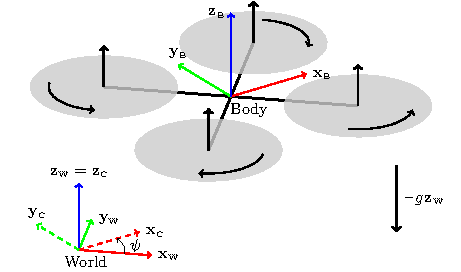
\includegraphics[width=0.8\textwidth]{img/quadrotor.pdf}
   \caption{Quadrotor with coordinate system and rotor forces.}
   \label{fig:quad}
\end{figure}

\subsection{Variables and Parameters}\label{sec:dynamicsvarpar}
Here we define some variables and parameters which we will use later
\begin{itemize}
	\item $m$ Mass of the quadrotor.
	\item $l$ Length of a quadrotor arm.
	\item $f_{i}$ Thrust produced by propeller $i$.
	\item $\kappa$ Torque constant relating rotor thrust to its drag torque
	\item $\bVec{c} = \sVec{0\\ 0\\ c} = \sVec{0\\ 0\\ \frac{1}{m} \Sigma f_i}$ Mass normalized, collective thrust of all the propellers.
	\item $M_{i}$ Drag torque produced by propeller $i$.
	\item $\bodytorques = \begin{bmatrix} \frac{\sqrt{2}}{2}l(f_1-f_2-f_3+f_4) \\
							\frac{\sqrt{2}}{2}l(-f_1-f_2+f_3+f_4) \\
							\kappa(f_1-f_2+f_3-f_4)
						\end{bmatrix}$ Torques acting on the body caused by the rotor thrusts.
	\item $\vect{\gravityvec}{\wfr}{} = \begin{bmatrix} 0 \\ 0 \\ -g \end{bmatrix}$ Gravitation vector in the world frame $\wfr$, where $\gravacc=9.81\unitfrac{m}{s^2}$.
	\item $\bVec{J} = \begin{bmatrix} J_{xx} & 0 & 0 \\ 0 & J_{yy} & 0 \\ 0 & 0 & J_{zz} \end{bmatrix} $ Moment of inertia matrix for rotations around the center of mass.
	\item $\vect{\pos}{\wfr}{\wfr \bfr} = \begin{bmatrix} x \\ y \\ z \end{bmatrix}$ Position of the quadrotor in the world frame $\wfr$.
	\item $\vect{\vel}{\wfr}{\wfr \bfr} = \begin{bmatrix} \dot{x} \\ \dot{y} \\ \dot{z} \end{bmatrix}$ Velocity of the quadrotor in the world frame $\wfr$.
	\item $\vect{\bodyrates}{\wfr}{\wfr \bfr} = \vect{\Omega}{\bfr}{} = \sVec{p \\ q\\ r} $  Angular velocity of the quadrotor in body coordinates $\bfr$. 
	Note that the $\bfr$ system is attached to the quadrotor body frame, hence $\vect{\bodyrates}{\wfr}{\wfr \bfr} = \vect{\Omega}{\bfr}{}$.
\end{itemize}

\subsection{Using Euler Angles}\label{sec:dynamicseuler}

In this section we use Euler angles and the corresponding rotation matrices as defined in Section~\ref{sec:traforotmat}, where the rotation matrix $\ori{\wfr \bfr}(\phi, \theta, \psi)$ is a function of the euler angles.
\newline\newline
We can evaluate~\eqref{eq:pdot_equal_F} in the world frame as
%
\begin{equation}
	\sVec{\ddot{x}\\ \ddot{y} \\ \ddot{z}} =  
\sVec{0\\ 0\\ - g} + \ori{\wfr \bfr}(\phi, \theta, \psi) \sVec{0\\ 0\\ c},
	\label{eq:lindynamics}
\end{equation}
%
or in vectorized form
%
\begin{equation}
	\ddot{\pos} = \vect{\gravityvec}{\wfr}{} + \ori{\wfr \bfr}(\phi, \theta, \psi) \cdot \bVec{c}.
\end{equation}
%
Next, we evaluate~\eqref{eq:ldot_equal_MS} in the body coordinate system $\bfr$
%
\begin{align}
	\begin{bmatrix} 
    	J_{xx} & 0 & 0 \\ 0 & J_{yy} & 0 \\ 0 & 0 & J_{zz} 
    \end{bmatrix}  
    \sVec{\dot{p}\\ \dot{q} \\ \dot{r}}  
    + 
	\sVec{p \\ q\\ r} 
	\times  
	\begin{bmatrix} 
		J_{xx} & 0 & 0 \\ 0 & J_{yy} & 0 \\ 0 & 0 & J_{zz} 
	\end{bmatrix} 
	\sVec{p \\ q\\ r} 
&= 
 \begin{bmatrix} \frac{\sqrt{2}}{2}l(f_1-f_2-f_3+f_4) \\
							\frac{\sqrt{2}}{2}l(-f_1-f_2+f_3+f_4) \\
							\kappa(f_1-f_2+f_3-f_4)
						\end{bmatrix} ,
\\
\begin{bmatrix} 
       J_{xx} \dot{p} + q \cdot r \left( J_{zz} - J_{yy} \right)\\
       J_{yy} \dot{q} + p \cdot r \left( J_{xx} - J_{zz} \right)\\
       J_{zz} \dot{r} + p \cdot q \left( J_{yy} - J_{xx} \right)
\end{bmatrix}   
  &= 
 \begin{bmatrix} \frac{\sqrt{2}}{2}l(f_1-f_2-f_3+f_4) \\
							\frac{\sqrt{2}}{2}l(-f_1-f_2+f_3+f_4) \\
							\kappa(f_1-f_2+f_3-f_4)
						\end{bmatrix},
\label{eq:rotdynamics}
\end{align}
%
or in vectorized form
%
\begin{equation}
	\bVec{J} \cdot \vectdot{\bodyrates}{\bfr}{\wfr \bfr} + \vect{\bodyrates}{\wfr}{\wfr \bfr} \times \bVec{J} \cdot   \vect{\bodyrates}{\wfr}{\wfr \bfr} = \bodytorques .
	\label{eq:rotdynamicsvector}
\end{equation}
%
Now, we want to write the quadrotor dynamics in state space form. 
First, we chose the state vector as
%
\begin{align}
	\bVec{s} &= \begin{bmatrix} x & y &z &\dot{x} &\dot{y} &\dot{z} &\phi &\theta &\psi &p &q &r \end{bmatrix}^{\top} ,\label{eq:state} \\
	&= \begin{bmatrix} \vect{\pos}{\wfr}{\wfr \bfr} & \vect{\vel}{\wfr}{\wfr \bfr} & \phi & \theta & \psi & \vect{\bodyrates}{\wfr}{\wfr \bfr} \end{bmatrix}^{\top} .
\end{align}
%
In the following we rewrite~\eqref{eq:lindynamics} and~\eqref{eq:rotdynamics} in order to fit the state space form. 
%
\begin{align}
\begin{bmatrix} 
	\dot{x} \\\dot{y} \\\dot{z} 
\end{bmatrix}
	&= \begin{bmatrix} 
	\dot{x} \\\dot{y} \\\dot{z} 
\end{bmatrix}, \\
%
\begin{bmatrix} 
	\ddot{x} \\\ddot{y} \\\ddot{z} 
\end{bmatrix}
	&= \begin{bmatrix} 0\\ 0\\ -g\end{bmatrix} + \ori{\wfr \bfr}(\phi, \theta, \psi) \begin{bmatrix} 0\\ 0\\ c \end{bmatrix},	\\
%
\begin{bmatrix}
	\dot{\phi} \\ \dot{\theta} \\ \dot{\psi} 
\end{bmatrix} 
 &=
\begin{bmatrix} 1 & \stan(\theta)\ssin(\phi) & \stan(\theta)\scos(\phi) \\ 
0 & \scos(\phi) & -\ssin(\phi) 
\\ 0 & \frac{\ssin(\phi)}{\scos(\theta)}  & \frac{\scos(\phi)}{\scos(\theta)} \end{bmatrix}    
\begin{bmatrix}
	p \\ q \\ r 
\end{bmatrix}, \label{eq:euleranglerates} \\
%
\begin{bmatrix} 
	\dot{p} \\\dot{q} \\\dot{r} 
\end{bmatrix}
	&= 
\begin{bmatrix} 
	\frac{1}{J_{xx}}
		\left( 
			\frac{\sqrt{2}}{2}l(f_1-f_2-f_3+f_4) 
			- q \cdot r \left( J_{zz} - J_{yy} \right)
		\right) \\
	\frac{1}{J_{yy}}
		\left( 
			\frac{\sqrt{2}}{2}l(-f_1-f_2+f_3+f_4)	
			- p \cdot r \left( J_{xx} - J_{zz} \right) 
		\right) \\
	\frac{1}{J_{zz}}
		\left( 
			\kappa(f_1-f_2+f_3-f_4)
			- q \cdot p \left( J_{yy} - J_{xx} \right)		 
		\right) \\
\end{bmatrix} ,
\end{align}
%
or in vectorized form
%
\begin{align}
	\vectdot{\pos}{\wfr}{\wfr \bfr} &= \vect{\vel}{\wfr}{\wfr \bfr}, \\
	\vectdot{\vel}{\wfr}{\wfr \bfr} &= \vect{\gravityvec}{\wfr}{} + \ori{\wfr \bfr}(\phi, \theta, \psi) \cdot \bVec{c}, \\
	\begin{bmatrix} \dot{\phi} \\ \dot{\theta} \\ \dot{\psi} \end{bmatrix} &=
	\begin{bmatrix} 1 & \stan(\theta)\ssin(\phi) & \stan(\theta)\scos(\phi) \\ 0 & \scos(\phi) & -\ssin(\phi) \\ 0 & \frac{\ssin(\phi)}{\scos(\theta)}  & \frac{\scos(\phi)}{\scos(\theta)} \end{bmatrix} \vect{\bodyrates}{\wfr}{\wfr \bfr}, \label{eq:eulerangleratesvectorized} \\
	\vectdot{\bodyrates}{\bfr}{\wfr \bfr} &= \bVec{J}^{-1} \cdot \left( \bodytorques - \vect{\bodyrates}{\wfr}{\wfr \bfr} \times \bVec{J} \cdot \vect{\bodyrates}{\bfr}{\wfr \bfr} \right).
\end{align}
%
Finally, the derivation of the Euler angle derivatives in~\eqref{eq:euleranglerates} and~\eqref{eq:eulerangleratesvectorized} is shown here. 
They are a function of the Euler angles and the body rates:
%
\begin{equation}
\begin{bmatrix} 
	\dot{\phi} \\\dot{\theta} \\\dot{\psi} 
\end{bmatrix}
= \begin{bmatrix} 
	\dot{\phi}(\phi,\theta,\psi,p,q,r) \\\dot{\theta}(\phi,\theta,\psi,p,q,r) \\\dot{\psi}(\phi,\theta,\psi,p,q,r) 
\end{bmatrix}.
\end{equation}
%
For this we use~\eqref{eq:B_omega_IB}:
%
\begin{equation}
\begin{bmatrix}
	p \\ q \\ r 
\end{bmatrix} 
 =
\begin{bmatrix}
	1 & 0 & -\ssin(\theta) \\
	0 & \scos(\phi) & \ssin(\phi)\scos(\theta) \\
	0 & -\ssin(\phi) & \scos(\phi)\scos(\theta)
\end{bmatrix} 
\begin{bmatrix}
	\dot{\phi}\\
	\dot{\theta}\\
	\dot{\psi}
\end{bmatrix} .
\label{eq:pqr_as_eulerangles}
\end{equation}
%
Inverting~\eqref{eq:pqr_as_eulerangles} finally leads to 
%
\begin{equation}
\begin{bmatrix}
	\dot{\phi} \\ \dot{\theta} \\ \dot{\psi} 
\end{bmatrix} 
 =
\begin{bmatrix} 1 & \stan(\theta)\ssin(\phi) & \stan(\theta)\scos(\phi) \\ 0 & \scos(\phi) & -\ssin(\phi) \\ 0 & \frac{\ssin(\phi)}{\scos(\theta)}  & \frac{\scos(\phi)}{\scos(\theta)} \end{bmatrix}
\begin{bmatrix}
	p \\ q \\ r 
\end{bmatrix} .     
\end{equation}



%\begin{bmatrix} 
%	\dot{x} \\\dot{y} \\\dot{z} 
%	\\\ddot{x} \\\ddot{y} \\\ddot{z} 
%	\\\dot{\Phi} \\\dot{\Theta} \\\dot{\Psi} 
%	\\\dot{p} \\\dot{q} \\\dot{r} \end{bmatrix}.


%For those who attended Mechanik III a refresh on Professor Glocker's notation
%\begin{itemize}
%\item Drall: $\vect{L}{}{O} $
%\item Impulsmoment: $ \ori{OS} \times \bVec{p} $
%\item Spin: $ \vect{I}{}{S} \cdot \bVec{\Omega} $
%\end{itemize}	

% Bibliography
%\bibliography{bibliography}{}
%\bibliographystyle{plain}

\subsection{Using Rotation Matrices}\label{sec:dynamicsrotmat}

We define $\ori{\wfr \bfr}$ to be the rotation matrix which transforms vectors from $\bfr$ to $\wfr$, but also describes the orientation of the quadrotor. 
In this section we will use the vectorized forms of the equations only.
\newline\newline
We can evaluate~\eqref{eq:pdot_equal_F} in the world frame as
%
\begin{equation}
	\ddot{\pos} = \vect{\gravityvec}{\wfr}{} + \ori{\wfr \bfr} \cdot \bVec{c}.
\label{eq:lindynamicsrotmat}
\end{equation}
%
Since we use the same representation of the body rates as in Section~\ref{sec:dynamicseuler}, the evaluation of~\eqref{eq:ldot_equal_MS} remains the same as in~\eqref{eq:rotdynamicsvector}.
\newline\newline
We chose the state vector as
%
\begin{equation}
	\bVec{s} = \begin{bmatrix} \vect{\pos}{\wfr}{\wfr \bfr} & \vect{\vel}{\wfr}{\wfr \bfr} & \ori{\wfr \bfr} & \vect{\bodyrates}{\wfr}{\wfr \bfr} \end{bmatrix}^{\top}.
\end{equation}
%
In the following, we rewrite~\eqref{eq:lindynamicsrotmat} and~\eqref{eq:rotdynamicsvector} in order to fit the state space form. 
%
\begin{align}
	\vectdot{\pos}{\wfr}{\wfr \bfr} &= \vect{\vel}{\wfr}{\wfr \bfr}, \\
	\vectdot{\vel}{\wfr}{\wfr \bfr} &= \vect{\gravityvec}{\wfr}{} + \ori{\wfr \bfr} \cdot \bVec{c},	\\
	\vectdot{\ori{}}{}{\wfr \bfr} &= \ori{\wfr \bfr} \cdot \vect{\hat{\bodyrates}}{\bfr}{\wfr \bfr}, \\
	\vectdot{\bodyrates}{\bfr}{\wfr \bfr} &= \bVec{J}^{-1} \cdot \left( \bodytorques - \vect{\bodyrates}{\wfr}{\wfr \bfr} \times \bVec{J} \cdot \vect{\bodyrates}{\wfr}{\wfr \bfr} \right).
\end{align}

\subsection{Using Quaternions} \label{sec:dyn_model_quat}

In this section, we use a quaternion $\vect{q}{}{\wfr \bfr}$, as defined in Section~\ref{sec:trafoquaternion}, to represent the orientation of the quadrotor. 
We will again use the vectorized forms of the equations only.
\newline\newline
We can evaluate~\eqref{eq:pdot_equal_F} in the world frame as
%
\begin{equation}
	\ddot{\pos} = \vect{\gravityvec}{\wfr}{} + \vect{q}{}{\wfr \bfr} \odot \bVec{c}.
	\label{eq:lindynamicsquat}
\end{equation}
%
Since we use the same representation of the body rates as in Section~\ref{sec:dynamicseuler}, the evaluation of~\eqref{eq:ldot_equal_MS} remains the same as in~\eqref{eq:rotdynamicsvector}.
\newline\newline
We chose the state vector as
%
\begin{equation}
	\bVec{s} = \begin{bmatrix} \vect{\pos}{\wfr}{\wfr \bfr} & \vect{\vel}{\wfr}{\wfr \bfr} & \vect{q}{}{\wfr \bfr} & \vect{\bodyrates}{\wfr}{\wfr \bfr} \end{bmatrix}^{\top}.
\end{equation}
%
In the following, we rewrite~\eqref{eq:lindynamicsquat} and~\eqref{eq:rotdynamicsvector} in order to fit the state space form.
%
\begin{align}
	\vectdot{\pos}{\wfr}{\wfr \bfr} &= \vect{\vel}{\wfr}{\wfr \bfr}, \\
	\vectdot{\vel}{\wfr}{\wfr \bfr} &= \vect{\gravityvec}{\wfr}{} + \vect{q}{}{\wfr \bfr} \odot \bVec{c},	\\
	\vectdot{q}{}{\wfr \bfr} &= \quatrot(\vect{\bodyrates}{\wfr}{\wfr \bfr}) \cdot \vect{q}{}{\wfr \bfr}, \label{eq:quatderivative} \\
	\vectdot{\bodyrates}{\bfr}{\wfr \bfr} &= \bVec{J}^{-1} \cdot \left( \bodytorques - \vect{\bodyrates}{\wfr}{\wfr \bfr} \times \bVec{J} \cdot \vect{\bodyrates}{\wfr}{\wfr \bfr} \right),
\end{align}
%
where
%
\begin{equation}
	\quatrot(\vect{\bodyrates}{\wfr}{\wfr \bfr}) = \frac{1}{2}
	\begin{bmatrix} 0 & -p & -q & -r \\ p & 0 & r & -q \\ q & -r & 0 & p \\ r & q & -p & 0 \end{bmatrix} 
	=
	\frac{1}{2}
	\bar{\bVec{Q}}
		\left( 	
			\begin{bmatrix}
				0\\
				\vect{\bodyrates}{\wfr}{\wfr \bfr}
			\end{bmatrix} 
		\right)
	=
	\frac{1}{2}
	\bar{\bVec{Q}}
		\left( 	
			\begin{bmatrix}
				0\\
				p \\ q \\ r
			\end{bmatrix} 
		\right).
\end{equation}
%
We find~\eqref{eq:quatderivative} by using~\eqref{eq:omega_from_q_body}
\begin{align}
\vectdot{q}{}{\wfr \bfr}
& = 
	\frac{1}{2}
	\vect{q}{}{\wfr \bfr} 
	\cdot	
	\begin{bmatrix}
		0\\
		\vect{\bodyrates}{\wfr}{\wfr \bfr}
	\end{bmatrix},
\\
& = 
	\frac{1}{2}
	\bar{\bVec{Q}}
		\left( 	
			\begin{bmatrix}
				0\\
				\vect{\bodyrates}{\wfr}{\wfr \bfr}
			\end{bmatrix} 
		\right)
	\vect{q}{}{\wfr \bfr} .
\end{align}
%
Equation~\eqref{eq:quatderivative} can be integrated as described in Appendix~\ref{sec:appquatint}.

\section{Control}

TODO: Adapt according to \cite{Faessler17ral} and \cite{Faessler18ral}.

This section describes our control algorithms that are used for OptiTrack based as well as for vision-based flying with our quadrotors.
The controller is split into a high-level part and a low-level part.
The high-level controller enables the quadrotor to track desired positions and velocities, whereas the low-level controller enables it to track desired attitudes or body rates.

\subsection{Control Structure Overview}

We can fly our quadrotors in two different set-ups namely when flying based only on on-board sensors (a camera and an IMU) and when flying in an OptiTrack motion capture system.
The schematics of the control architecture for vision based flight are illustrated in Fig.~\ref{fig:vision_based_contr_schem}.
In vision based flight, all the state estimation and high-level control runs on the Odroid which sends attitude commands to the PX4.
In this setting, the user laptop is only used for feedback and some very high level inputs.

The schematics of the control architecture for OptiTrack based flight are illustrated in Fig.~\ref{fig:optitrack_based_contr_schem}.
In OptiTrack based flight, the Odroid only serves as a relay for feedback from the PX4 via the WiFi link.
In this setting, the user laptop receives pose measurements from the OptiTrack and uses them to compute a state estimate.
To compensate for the round trip delay from when a pose was measured until the corresponding control command is received on the quadrotor, we also predict the state forward in time to compensate for this delay.
This predicted state is then used on the laptop to compute body rate commands which are sent through Laird modules directly to the PX4.

\subsection{Nomenclature}

When describing the control and state estimation, we make use of some notation that we introduce here for clarity.
We use a hat (e.g. $\hat{v}$) and a tilde (e.g. $\tilde{v}$) to denote an estimated and measured value, respectively.
To describe the multiplication of two quaternions $\bVec{q}_1$ and $\bVec{q}_2$ we write $\bVec{q}_1 \otimes \bVec{q}_2$, and we write $\bVec{q} \odot \bVec{v}$ for the rotation of a vector $\bVec{v}$ by the quaternion $\bVec{q}$.
Furthermore, we express the basis vectors of a coordinate system as e.g. $\vect{x}{}{\bfr}$ which denotes the $x$-basis vector of the body coordinate system, as illustrated in Fig.~\ref{fig:quad}.
A prescript (e.g. $\prescript{}{\bfr}{\bVec{v}}$) indicates that the vector $\bVec{v}$ is expressed in the body coordinate system. 
In this section, for simplicity, vectors that are expressed in world coordinates do not have prescripts with the exception of the body rates $\bomega$, which are always expressed in body coordinates.

\subsection{Summary of the used Dynamical Model} \label{sec:dynamics}

For state estimation and control, we make use of the following dynamical model (as derived in Section~\ref{sec:dyn_model_quat}) for our quadrotor:
%
\begin{align}
	\dot{\ori{}} &= \bVec{v}, \label{eq:dynamics_1} \\
	\dot{\bVec{v}} &= \bVec{g} + \bVec{q} \odot \bVec{c},\label{eq:dynamics_2}	\\
	\dot{\bVec{q}} &= \quatrot(\bomega) \cdot \bVec{q}, \label{eq:dynamics_3}\\
	\dot{\bomega} &= \bVec{J}^{-1} \cdot \left( \bodytorques - \bomega \times \bVec{J} \cdot \bomega \right) \label{eq:dynamics_4},
\end{align}
%
where $\ori{} = [x \; y \; z]^{\top}$ and $\bVec{v} = [v_x \; v_y \; v_z]^{\top}$ are the position and velocity in world coordinates, $\bVec{q} = [q_w \; q_x \; q_y \; q_z]^{\top}$ is the orientation of the quadrotor's body coordinates with respect to the world coordinates, and $\bomega = [p \; q \; r]^{\top}$ denotes the body rates (roll, pitch and yaw, respectively) expressed in body coordinates. 
The skew-symmetric matrix $\quatrot(\bomega)$ is defined as
%
\begin{equation}
	\quatrot(\bomega) = \frac{1}{2}
	\begin{bmatrix} 0 & -p & -q & -r \\ p & 0 & r & -q \\ q & -r & 0 & p \\ r & q & -p & 0 \end{bmatrix}.
\end{equation}
%
We define the gravity vector as $\bVec{g} = [0 \; 0 \; -g]^{\top}$ with $g = \SI{9.81}{\meter \per \second \squared}$ and the second-order moment-of-inertia matrix of the quadrotor as $\bVec{J} = \diag{J_{xx}, \; J_{yy}, \; J_{zz}}$.
The mass-normalized thrust vector is $\bVec{c} = [0 \; 0 \; c]^{\top}$, with
\begin{equation}
	m c = f_1 + f_2 + f_3 + f_4,
	\label{eq:col_thrust}
\end{equation}
where $m$ is the mass of the quadrotor and $f_{i}$ are the four motor thrusts as illustrated in Fig.~\ref{fig:quad}.
The torque inputs $\bodytorques$ are composed of the single-rotor thrusts as

\begin{equation}
	\bodytorques = \begin{bmatrix} \frac{\sqrt{2}}{2}l(f_1-f_2-f_3+f_4) \\
							\frac{\sqrt{2}}{2}l(-f_1-f_2+f_3+f_4) \\
							\kappa(f_1-f_2+f_3-f_4)
						\end{bmatrix},
	\label{eq:body_torques}
\end{equation}
%
where $l$ is the quadrotor arm length and $\kappa$ is the rotor-torque coefficient. 
Our coordinate-system conventions and rotor numbering are illustrated in Fig.~\ref{fig:quad}.

\subsection{High-Level Control}

TODO: Control from \cite{Faessler18ral}, reference to TR \cite{Faessler17tr}.

The high-level controller takes a reference state as input and computes the desired attitude or desired body rates, which are then sent to the low-level controller.
A reference state consists of a reference position $\posRef$, a reference velocity $\velRef$, a reference acceleration $\accRef$, and a reference heading $\yawRef$.
First, we describe the position controller, followed by the attitude controller. 
The two high-level control loops are synchronized and run at \SI{50}{\Hz}.

\subsubsection{Position Controller} \label{sec::Position_Controller}

To track a reference trajectory, we implemented a PD controller with feed-forward terms on the reference acceleration from the sampled trajectory and gravity:
%
\begin{equation}
	\accDes{} = 
	\bVec{P}_{pos}
	\cdot
	\left(
		\posRef - \posEst
	\right)
	+
	\bVec{D}_{pos}
	\cdot
	\left(
		\velRef - \velEst
	\right)
	+\accRef
	-\bVec{g},
	\label{eq:position_controller}
\end{equation}
%
with gain matrices $\bVec{P}_{pos}=\diag{p_{xy},p_{xy},p_{z}}$ and $\bVec{D}_{pos} = \diag{d_{xy},d_{xy},d_{z}}$.
To compute the desired normalized thrust $c_{des}$, we project the desired acceleration onto the current $\prescript{}{\wfr}{\bVec{e}}_{z}^{\bfr}$ axis
%
\begin{equation}
	c_{des} = \bVec{a}_{des} \cdot \bVec{e}_{z}^B.
	\label{eq:norm_thrust}
\end{equation}
%
The output of the position controller is the desired accelerations $\accDes{}$.
The desired acceleration, together with the reference heading $\yawRef$, encodes the desired orientation as well as a mass normalized thrust $c_{des}$.

\subsubsection{Attitude Controller} \label{sec::attitude_controller}

Since a quadrotor can only accelerate in its body $z$ direction, $\accDes{}$ enforces two degrees of freedom of the desired attitude.
The third degree of freedom is enforced by reference heading $\yawRef$.
Note that the rotation around the body $z$ axis has no influence on the translational behaviour of the quadrotor.
Therefore, we want to align the body $z$ axis with the desired acceleration $\accDes{}$ by rotating around the body $x$ and $y$ axes and use rotations around the body $z$ axis only to control the heading.
Our quadrotors have much more attitude control authority on the $x$ and $y$ axes than on the $z$ axis because there, they can make use of thrust differences as opposed to differences in rotor drag torques.
The moment due to the maximum-possible thrust difference is much larger than the maximum possible difference of rotor drag torques.
For this reason, we separate the attitude control into two parts as described in the following.

\subsubsection*{Desired Roll and Pitch Rates} \label{sec:roll_pitch_control}

From the current attitude estimate and the desired acceleration, we can compute the current and the desired body $z$ axis, respectively, as
%
\begin{align}
	\hat{\bVec{e}}_{z}^{\bfr} &= \hat{\bVec{q}} \odot [0 \; 0 \; 1]^{\top}, \\
	\bVec{e}_{z,des}^{\bfr} &= \frac{\accDes{}}{\norm{\accDes{}}}.
\end{align}
%
Now, we design an error quaternion that describes the necessary rotation to align these two vectors.
To do so, we compute the angle $\alpha$ between the two vectors and a normal vector $\bVec{n}$ to both of them:
%
\begin{align}
	\alpha &= \arccos(\hat{\bVec{e}}_{z}^{\bfr} \cdot \bVec{e}_{z,des}^{\bfr}), \\
	\bVec{n} &= \frac{\hat{\bVec{e}}_{z}^{\bfr} \times \bVec{e}_{z,des}^{\bfr}}
					{\norm{\hat{\bVec{e}}_{z}^{\bfr} \times \bVec{e}_{z,des}^{\bfr}}},
\end{align}
%
where $\bVec{n}$, $\alpha$ are the rotation axis and angle of the error quaternion.
Since we want to apply this rotation with respect to the current body orientation, we have to transform the rotation axis $\bVec{n}$ into body coordinates using the current attitude estimate $\hat{\bVec{q}}$
%
\begin{equation}
	\prescript{}{\bfr}{\bVec{n}} = \hat{\bVec{q}}^{-1} \odot \bVec{n}.
\end{equation}
%
The error quaternion can then be constructed as
%
\begin{equation}	
	\bVec{q}_{e,rp} = \begin{bmatrix} 
			\cos(\frac{\alpha}{2}) \\  
			\prescript{}{\bfr}{\bVec{n}} \sin(\frac{\alpha}{2})
		\end{bmatrix}.
\end{equation}
%
Note that if $\alpha = 0$, the rotation axis is undetermined and we set the error quaternion $\bVec{q}_{e,rp}$ to be the identity directly.
Also note that by construction, the $z$ component of $\bVec{q}_{e,rp}$ is always zero, which assures that no rotation around the body $z$ axis is necessary to align $\hat{\bVec{e}}_{z}^{\bfr}$ with $\bVec{e}_{z,des}^{\bfr}$.
From the error quaternion $\bVec{q}_{e,rp}$, we can then compute the desired roll and pitch rates with the following control law:
%
\begin{equation}
	\begin{bmatrix} p \\ q \end{bmatrix}_{des} = \begin{cases} 2 \cdot p_{rp} \cdot \bVec{q}_{e,rp}^{(x,y)} &\mbox{if } \bVec{q}_{e,rp}^{(w)} \geq 0 \\
						- 2 \cdot p_{rp} \cdot \bVec{q}_{e,rp}^{(x,y)} &\mbox{if } \bVec{q}_{e,rp}^{(w)} < 0 
					\end{cases}.
\end{equation}
%
It can be shown that this control law is globally asymptotically stable and its discrete implementation is robust to measurement noise~\cite{Brescianini13tr, Mayhew11ac}.

\subsubsection*{Desired Yaw Rate} \label{sec:yaw_control}

\begin{figure}[t]
   \centering
   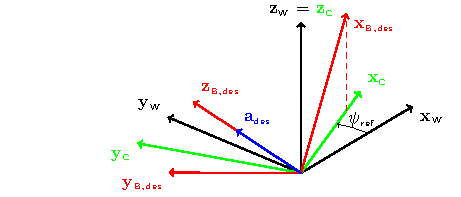
\includegraphics[width=0.8\textwidth]{img/coordinate_systems.pdf}
   \caption{Coordinate frames used in the attitude controller.
  We make use of the coordinate frame $C$, which is obtained by rotating the world frame ($\wfr$) by the reference heading $\yawRef$ to construct, together with the desired acceleration $\bVec{a}_{des}$, the full desired orientation of the body frame ($\bfr$).}
   \label{fig:att_cont_frames}
\end{figure}

To compute the desired yaw rate $r_{des}$, we look at the heading error that remains after aligning $\hat{\bVec{e}}_{z}^{\bfr}$ with $\bVec{e}_{z,des}^{\bfr}$ with the above control law.
To do so, we first compute the full desired attitude.
For this, we make use of an intermediate coordinate system $C$, which is the world frame rotated around its $z$ axis by the desired heading $\yawRef$ as illustrated in Fig.~\ref{fig:att_cont_frames}.
The $x$ and $y$ axes of the coordinate system $C$ are defined as
%
\begin{align}
	\bVec{e}_{x}^{C} &= [\cos(\yawRef) \; \sin(\yawRef) \; 0]^{\top}, \\
	\bVec{e}_{y}^{C} &= [-\sin(\yawRef) \; \cos(\yawRef) \; 0]^{\top}.
\end{align}
%
The goal of rotating around the quadrotor's $z$ axis is to align the projection of its $x$ axis onto the world $x-y$ plane with $\bVec{e}_{x}^{C}$.
This forces the desired body $x$ axis $\bVec{e}_{x,des}^{\bfr}$ to lie in a plane spanned by $\bVec{e}_{x}^{C}$ and $\bVec{e}_{x}^{\wfr}$, which is fulfilled by
%
\begin{equation}
	\bVec{e}_{x,des}^{\bfr} = \frac{\bVec{e}_{y}^{C} \times \bVec{e}_{z,des}^{\bfr}}
								{\norm{\bVec{e}_{y}^{C} \times \bVec{e}_{z,des}^{\bfr}}}.
\end{equation}
%
Note that if this cross product is zero, there are infinitely many rotations around the desired body $z$ axis that achieve the desired heading.
Therefore, in that case, we apply a desired yaw rate $r = 0$.
\newline\newline
If the desired body $z$ axis has a negative $z$ component (i.e. $\bVec{e}_{z,des}^{\bfr}$ is pointing downwards), the projection of the computed desired body $x$ axis into the horizontal plane will point in the opposite direction of $\bVec{e}_{x}^{C}$, therefore we use the negation of it.
From $\bVec{e}_{x,des}^{\bfr}$ and $\bVec{e}_{z,des}^{\bfr}$, we can then compute $\bVec{e}_{y,des}^{\bfr}$ as
%
\begin{equation}
	\bVec{e}_{y,des}^{\bfr} = \frac{\bVec{e}_{z,des}^{\bfr} \times \bVec{e}_{x,des}^{\bfr}}
								{\norm{\bVec{e}_{z,des}^{\bfr} \times \bVec{e}_{x,des}^{\bfr}}}.
\end{equation}
%
Now, the full desired attitude $\bVec{q}_{des}$ can be built from the three desired body axes $\bVec{e}_{x,des}^{\bfr}$, $\bVec{e}_{y,des}^{\bfr}$ and $\bVec{e}_{z,des}^{\bfr}$.
Our definition of the heading has the advantage of being meaningful for any orientation of the quadrotor, which is not the case, for instance, when using a definition based on Euler angles.
From this, we can then compute an error quaternion that describes the necessary rotation to achieve the full desired attitude after rotating by $\bVec{q}_{e,rp}$ as
%
\begin{equation}
	\bVec{q}_{e,y} = (\hat{\bVec{q}} \otimes \bVec{q}_{e,rp})^{-1} \otimes \bVec{q}_{des}.
\end{equation}
%
Note that the $x$ and $y$ components of $\bVec{q}_{e,y}$ are always zero.
Similarly to the desired roll and pitch rate, we can now compute the desired yaw rate from $\bVec{q}_{e,y}^{(z)}$ with a gain $p_{yaw}$ as
%
\begin{equation}
	r_{des} = \begin{cases} 2 \cdot p_{yaw} \cdot \bVec{q}_{e,y}^{(z)} &\mbox{if } \bVec{q}_{e,y}^{(w)} \geq 0 \\
						- 2 \cdot p_{yaw} \cdot \bVec{q}_{e,y}^{(z)} &\mbox{if } \bVec{q}_{e,y}^{(w)} < 0 
					\end{cases}.
\end{equation}
%
Splitting the attitude control into these two parts allows us to have different gains for $p_{rp}$ and $p_{yaw}$, which is desirable due to different control limits.

\subsection{Low-Level Control} \label{sec:low_level_cont}

TODO: Update to \cite{Faessler17ral}.

The commands sent to the low-level control on the PX4 are the desired body rates $\bomega_{des}$ and the desired mass-normalized thrust $c_{des}$.
From the desired body rates $\bomega_{des}$ and the measured body rates $\tilde{\bomega}$, we can compute the desired torques $\bodytorques_{des}$ with a feedback linearizing control scheme:
%
\begin{equation}
	\bodytorques_{des}
	= \bVec{J} \cdot \bVec{P}_{att} \cdot \left( \bomega_{des} - \hat{\bomega} \right)
	+ \hat{\bomega} \times \bVec{J} \cdot \hat{\bomega},
\end{equation}
%
where $\bVec{P}_{att}=\diag{p_{pq},p_{pq},p_{r}}$.
Then, we can substitute $\bodytorques_{des}$ and $c_{des}$ into~\eqref{eq:body_torques} and~\eqref{eq:col_thrust} and solve them for the desired nominal rotor thrusts (see Section~\ref{sec:self_calibration}) that must be applied:
%
\begin{equation}
	\begin{bmatrix}
		\check{f}_1 \\ \check{f}_2\\ \check{f}_3 \\ \check{f}_4
	\end{bmatrix}
	= 
	\begin{bmatrix}
		\frac{1}{4 \lambda_1} \cdot \left(m \cdot c_{des} + \frac{1}{\kappa} \cdot \bodytorques_{des}^{y} - \frac{\sqrt{2}}{l} \cdot \bodytorques_{des}^{p} + \frac{\sqrt{2}}{l} \cdot \bodytorques_{des}^{r} \right) \\
 \frac{1}{4 \lambda_2} \cdot \left(m \cdot c_{des} - \frac{1}{\kappa} \cdot \bodytorques_{des}^{y} - \frac{\sqrt{2}}{l} \cdot \bodytorques_{des}^{p} - \frac{\sqrt{2}}{l} \cdot \bodytorques_{des}^{r} \right) \\
  \frac{1}{4 \lambda_3} \cdot \left(m \cdot c_{des} + \frac{1}{\kappa} \cdot \bodytorques_{des}^{y} + \frac{\sqrt{2}}{l} \cdot \bodytorques_{des}^{p} - \frac{\sqrt{2}}{l} \cdot \bodytorques_{des}^{r} \right) \\
  \frac{1}{4 \lambda_4} \cdot \left(m \cdot c_{des} - \frac{1}{\kappa} \cdot \bodytorques_{des}^{y} + \frac{\sqrt{2}}{l} \cdot \bodytorques_{des}^{p} + \frac{\sqrt{2}}{l} \cdot \bodytorques_{des}^{r} \right)
	\end{bmatrix} ,
\end{equation}
%
with $\kappa$ being the rotor-torque coefficient and $\lambda_i$ being the rotor fitness coefficients as described in Section~\ref{sec:self_calibration}.

\subsubsection{Rotor Thrusts Saturation}

TODO: Describe how we saturate the single rotor thrusts according to \cite{Faessler17ral}.

\subsection{Delay Compensation}

TODO: about state predictor

\section{Trajectory Generation}

\subsection{Computing Relevant Maxima from a Reference State}

When designing a trajectory, it is often desired to enforce some limits which need to be computed from a desired state.
This section shows how to compute to most relevant values for quadrotors, namely the speed, the collective thrust, and the norm of the roll and pitch rates (especially relevant for vision-based quadrotors).
We assume that from a sample point on a given trajectory, we can get the reference state $\bVec{s}_{des}$ containing the position, velocity, acceleration, and jerk.
%
\begin{equation}
	\bVec{s}_{des} = \begin{bmatrix} \ori{des} & \bVec{v}_{des} & \bVec{a}_{des} & \bVec{j}_{des} \end{bmatrix}
\end{equation}

\paragraph{Speed and Collective Thrust\newline\newline}
The speed can simply be obtained by taking the norm of the reference velocity
%
\begin{equation}
	v = \norm{\bVec{v}_{des}},
\end{equation}
%
and the collective thrust can be computed as
%
\begin{equation}
	c = \norm{\bVec{a}_{des} - \bVec{g}},
\end{equation}
%
with $\bVec{g} = [0 \; 0 \; -g]^{\top}$.

\paragraph{Roll and Pitch Rate Norm\newline\newline}

We introduce the desired acceleration vector in world coordinates as
%
\begin{equation}
	\bVec{f} = \bVec{a}_{des} - \bVec{g} = \ori{WB} \cdot \begin{bmatrix}
		0 \\ 0 \\ c
	\end{bmatrix} = \ori{WB} \cdot \bVec{c},
\end{equation}
%
where $\bVec{g}$ is defined as above.
Note that $\norm{\bVec{f}} = c$ since the rotation of a vector does not change is length.
Therefore we can say
%
\begin{equation}
	\ori{WB} \cdot \begin{bmatrix}
		0 \\ 0 \\ 1
	\end{bmatrix} = \frac{\bVec{f}}{\norm{\bVec{f}}} = \bar{\bVec{f}}.
\end{equation}
%
Taking the derivative leads to
%
\begin{align}
	\ori{WB} \cdot \hat{\bomega} \cdot \begin{bmatrix}
		0 \\ 0 \\ 1
	\end{bmatrix} &= \dot{\bar{\bVec{f}}}, \\
	\hat{\bomega} \cdot \begin{bmatrix}
		0 \\ 0 \\ 1
	\end{bmatrix} &= \ori{WB}^{\top} \cdot \dot{\bar{\bVec{f}}}, \\
	\begin{bmatrix}
		\omega_y \\ -\omega_x \\ 0
	\end{bmatrix} &= \ori{WB}^{\top} \cdot \dot{\bar{\bVec{f}}},
\end{align}
%
where $\dot{\bar{\bVec{f}}}$ is computed as
%
\begin{align}
	\dot{\bar{\bVec{f}}} &= \frac{d}{dt} \left( \frac{\bVec{f}}{\norm{\bVec{f}}} \right), \\
	&= \frac{\dot{\bVec{f}} \cdot \norm{\bVec{f}} - \bVec{f} \cdot \frac{\bVec{f}^{\top} \cdot \dot{\bVec{f}}}{\norm{\bVec{f}}}}{\norm{\bVec{f}}^2}, \\
	&= \frac{\dot{\bVec{f}}}{\norm{\bVec{f}}} - \frac{\bVec{f} \cdot \bVec{f}^{\top} \cdot \dot{\bVec{f}}}{\norm{\bVec{f}}^3}, \\ 
	&= \frac{\bVec{j}}{\norm{\bVec{f}}} - \frac{\bVec{f} \cdot \bVec{f}^{\top} \cdot \bVec{j}}{\norm{\bVec{f}}^3},
\end{align}
%
using the fact that $\dot{\bVec{f}} = \bVec{j}$.
With all this we can write
\begin{align}
	\begin{bmatrix}
		\omega_y \\ -\omega_x \\ 0
	\end{bmatrix} &= \ori{WB}^{\top} \cdot \left( \frac{\bVec{j}}{\norm{\bVec{f}}} - \frac{\bVec{f} \cdot \bVec{f}^{\top} \cdot \bVec{j}}{\norm{\bVec{f}}^3} \right), \\
	&= \ori{WB}^{\top} \cdot \frac{\bVec{j}}{c} - \ori{WB}^{\top} \frac{\ori{WB} \cdot \bVec{c} \cdot \bVec{c}^{\top} \cdot \ori{WB}^{\top} \cdot \bVec{j}}{c^3}, \\
	&= \ori{WB}^{\top} \cdot \frac{\bVec{j}}{c} - \frac{\bVec{c} \cdot \bVec{c}^{\top} \cdot \ori{WB}^{\top} \cdot \bVec{j}}{c^3}.
\end{align}
%
Noting that
\begin{equation}
	\bVec{c} \cdot \bVec{c}^{\top} = \begin{bmatrix}
		0 & 0 & 0 \\
		0 & 0 & 0 \\
		0 & 0 & c^2
	\end{bmatrix},
\end{equation}
%
and using~\eqref{eq:r_basis_vectors}, we get
%
\begin{equation}
	\begin{bmatrix}
		\omega_y \\ -\omega_x \\ 0
	\end{bmatrix} = \begin{bmatrix}
		(\bVec{e}_x^B)^{\top} \cdot \frac{\bVec{j}}{c} \\
		(\bVec{e}_y^B)^{\top} \cdot \frac{\bVec{j}}{c} \\
		(\bVec{e}_z^B)^{\top} \cdot \frac{\bVec{j}}{c}
	\end{bmatrix} -
	\begin{bmatrix}
		0 \\
		0 \\
		(\bVec{e}_z^B)^{\top} \cdot \frac{\bVec{j}}{c}
	\end{bmatrix}.
\end{equation}
% 
Note that $\norm{\ori{WB}^{\top} \cdot \frac{\bVec{j}}{c}} = \norm{\frac{\bVec{j}}{c}}$ and that $\bVec{e}_z^B$ can be retrieved from the desired acceleration as
%
\begin{equation}
	\bVec{e}_z^B = \frac{\bVec{a}_{des} - \bVec{g}}{\norm{\bVec{a}_{des} - \bVec{g}}}.
\end{equation}
%
Therefore, we can compute the norm of the roll and pitch body rates as
%
\begin{equation}
	\norm{\omega_{x,y}} = \norm{\begin{bmatrix}
		\omega_y \\ -\omega_x \\ 0
	\end{bmatrix}} = \sqrt{\norm{\frac{\bVec{j}}{c}}^2 - \left( (\bVec{e}_z^B)^{\top} \cdot \frac{\bVec{j}}{c} \right)^2}
\end{equation}

%%%%%%%%%%%%%%%%%%%%%%%%%%%%%%%%%%%%%%%%%%%%%
% Appendix
%%%%%%%%%%%%%%%%%%%%%%%%%%%%%%%%%%%%%%%%%%%%%
\newpage
\appendix
\appendixpage
\addappheadtotoc

\section{Zeroth Order Integration of a Unit Quaternion} \label{sec:appquatint}

Simply integrating a quaternion derivative component-wise does not guarantee to result in a unit quaternion and requires normalization. 
Under the assumption of a discrete time step in the interval $[t, t+\Delta t]$ with constant body rates $\vect{\bodyrates}{\wfr}{\wfr \bfr}$, a nice solution for the integration exists (from~\cite{Trawny05tr}) which does not require to normalize the quaternion. 
%
First we restate~\eqref{eq:quatderivative}
%
\begin{equation}
	\vectdot{q}{}{\wfr \bfr} = \quatrot(\vect{\bodyrates}{\wfr}{\wfr \bfr}) \cdot \vect{q}{}{\wfr \bfr}.
\end{equation}
%
In literature we find the solution to this differential equation with starting point $\vect{q}{}{\wfr \bfr}(t)$ to be 
%
\begin{equation}
	\vect{q}{}{\wfr \bfr}(t + \Delta t) = e^{\left( \quatrot(\vect{\bodyrates}{\wfr}{\wfr \bfr}) \Delta t \right)} \cdot \vect{q}{}{\wfr \bfr}(t).
\end{equation}
%
The matrix exponential is defined as
%
\begin{equation}
	e^{\left( \quatrot(\vect{\bodyrates}{\wfr}{\wfr \bfr}) \Delta t \right)} = 
	\bVec{I}_4 \; + \; \quatrot(\vect{\bodyrates}{\wfr}{\wfr \bfr}) \cdot \Delta t \; + \; \frac{1}{2!} \left( \quatrot(\vect{\bodyrates}{\wfr}{\wfr \bfr}) \cdot \Delta t \right)^2 \; + \; \frac{1}{3!} \left( \quatrot(\vect{\bodyrates}{\wfr}{\wfr \bfr}) \cdot \Delta t \right)^3 \; + \; \ldots
	\label{eq:matrixexponential}
\end{equation}
%
It can easily be verified that
%
\begin{equation}
	\left( \quatrot(\vect{\bodyrates}{\wfr}{\wfr \bfr}) \right)^2 = - \frac{1}{4} \lVert \vect{\bodyrates}{\wfr}{\wfr \bfr}\rVert^2 \cdot \bVec{I}_4,
	\label{eq:quatrotsquare}
\end{equation}
%
where
%
\begin{equation}
	\lVert \vect{\bodyrates}{\wfr}{\wfr \bfr}\rVert = \sqrt{p^2 + q^2 + r^2}.
\end{equation}
%
Using~\eqref{eq:quatrotsquare} and rearranging the terms, \eqref{eq:matrixexponential} can be written as
%
\begin{align}
	e^{\left( \quatrot(\vect{\bodyrates}{\wfr}{\wfr \bfr}) \Delta t \right)} 
	&= 
	\bVec{I}_4 \cdot 
	\left( 
		1 
		- \frac{\left( \lVert \vect{\bodyrates}{\wfr}{\wfr \bfr}\rVert \frac{\Delta t}{2} \right)^2}{2!} 
		+ \frac{\left( \lVert \vect{\bodyrates}{\wfr}{\wfr \bfr}\rVert \frac{\Delta t}{2} \right)^4}{4!} 
		- \ldots 
	\right), \\
	& \quad 
	+ \frac{2}{\lVert \vect{\bodyrates}{\wfr}{\wfr \bfr}\rVert} \quatrot(\vect{\bodyrates}{\wfr}{\wfr \bfr}) \cdot 	
	\left( 
		\frac{\left( \lVert \vect{\bodyrates}{\wfr}{\wfr \bfr}\rVert \frac{\Delta t}{2} \right)}{1!} 
		- \frac{\left( \lVert \vect{\bodyrates}{\wfr}{\wfr \bfr}\rVert \frac{\Delta t}{2} \right)^3}{3!} 
		+  \ldots 
	\right), \nonumber \\
	&= \bVec{I}_4 \cdot \cos{\left( \frac{\lVert \vect{\bodyrates}{\wfr}{\wfr \bfr}\rVert \Delta t}{2} \right)} + \frac{2}{\lVert \vect{\bodyrates}{\wfr}{\wfr \bfr}\rVert} \cdot \quatrot(\vect{\bodyrates}{\wfr}{\wfr \bfr}) \cdot \sin{\left( \frac{\lVert \vect{\bodyrates}{\wfr}{\wfr \bfr}\rVert \Delta t}{2} \right)}.
\end{align}
%
So the state update of the quaternion becomes
%
\begin{equation}
	\vect{q}{}{\wfr \bfr}(t + \Delta t) = \left( \bVec{I}_4 \cdot \cos{\left( \frac{\lVert \vect{\bodyrates}{\wfr}{\wfr \bfr}\rVert \Delta t}{2} \right)} + \frac{2}{\lVert \vect{\bodyrates}{\wfr}{\wfr \bfr}\rVert} \cdot \quatrot(\vect{\bodyrates}{\wfr}{\wfr \bfr}) \cdot \sin{\left( \frac{\lVert \vect{\bodyrates}{\wfr}{\wfr \bfr}\rVert \Delta t}{2} \right)} \right) \cdot \vect{q}{}{\wfr \bfr}(t) .
\end{equation}

\section{Differentiating the Angular Momentum}

This section shows how to differentiate $ \vect{L}{}{O} $.
First, we restate~\eqref{eq:L_O_S} for the definition of the angular momentum
%
\begin{equation}
	\vect{L}{}{O} = \ori{OS} \times \bVec{p} + \vect{I}{}{S} \cdot \bVec{\Omega} .
	\label{eq:L_O_S_2}
\end{equation}
%
Later we will use Euler's differentiation rule, therefore we restate it here. 
Euler's differentiation rule is used to differentiate in a body fixed coordinate system $\bfr$
%
\begin{equation}
	\vectdot{c}{\bfr}{} =
	\left( \vect{\thrust}{\bfr}{} \right)' + \vect{\bodyrates}{\wfr}{\wfr \bfr}  \times \vect{\thrust}{\bfr}{} .
	\label{eq:app_euler_rule}
\end{equation}
%
Note the special notation for $ \left( \vect{\thrust}{\bfr}{} \right)' $ which is just the  differentiation over time of $ \vect{\thrust}{\bfr}{} $ which is different than the differentiation expressed in the $\bfr$ system $ \vectdot{c}{\bfr}{} $.
Now, lets start to calculate $\vectdot{L}{}{O}$. 
For better readability we differentiate the two terms in~\eqref{eq:L_O_S_2} separately:
%
\begin{align}
	\dot{ \left( \ori{OS} \times \bVec{p} \right) } & = 
	\vectdot{\ori{}}{}{OS} \times \bVec{p} + 
	\ori{OS} \times \dot{ \bVec{p} }, \\
	& = 
	v_{S} \times \bVec{p} +
	\ori{OS} \times \dot{ \bVec{p} }, \\
	& = 
	v_{S} \times m \cdot v_{S} + 
	\ori{OS} \times \dot{ \bVec{p} }, \\
	& = 
	\ori{OS} \times \dot{ \bVec{p} }.
	\label{eq:appendix_drall_deriv0}
\end{align}
%
To differentiate $ \vect{I}{}{S} \cdot \bVec{\Omega} $ we evaluate it in the body fixed coordinate system $\bfr$. 
We do this because the second moment of inertia matrix $\vect{I}{B}{S}$ is constant in a body fixed frame
%
\begin{align}
	\prescript{}{\bfr}{\dot{ \left( \vect{I}{}{S} \cdot \bVec{\Omega} \right)} } 
	& =
	\left( \vect{I}{B}{S} \vect{\Omega}{\bfr}{} \right)'
	+ \vect{\Omega}{\bfr}{} \times \vect{I}{B}{S} \cdot \vect{\Omega}{\bfr}{}, \\
	& = 
	\cancelto{0}{\left( \vect{I}{B}{S}  \right)'} \vect{\Omega}{\bfr}{} +
	 \vect{I}{B}{S}  \left( \vect{\Omega}{\bfr}{} \right)'
	+ \vect{\Omega}{\bfr}{} \times \vect{I}{B}{S} \cdot \vect{\Omega}{\bfr}{}, \\
	& = 
	\vect{I}{B}{S}  \left( \vect{\Omega}{\bfr}{} \right)'
	+ \vect{\Omega}{\bfr}{} \times \vect{I}{B}{S} \cdot \vect{\Omega}{\bfr}{}.
	\label{eq:appendix_drall_deriv1}
\end{align}
%
To rewrite $ \left( \vect{\Omega}{\bfr}{} \right)' $ we differentiate the angular velocity of the body using euler's formula~\eqref{eq:app_euler_rule}
%
\begin{align}
	\vectdot{\Omega}{\bfr}{}
	&=
	\left( \vect{\Omega}{\bfr}{} \right)' + 
	\vect{\bodyrates}{\wfr}{\wfr \bfr}  \times \vect{\Omega}{\bfr}{}, \\
	&= 	
	\left( \vect{\Omega}{\bfr}{} \right)' + 
	\cancelto{0}{ \vect{\Omega}{\bfr}{}  \times \vect{\Omega}{\bfr}{} }, \\
	&=
	\left( \vect{\Omega}{\bfr}{} \right)'. \label{eq:app_body_rates_dev}
\end{align}
%
Inserting~\eqref{eq:app_body_rates_dev} in~\eqref{eq:appendix_drall_deriv1} we can continue with the differentiation of the second term
%
\begin{align}
	\prescript{}{\bfr}{\dot{ \left( \vect{I}{}{S} \cdot \bVec{\Omega} \right) }}
	& =
	\vect{I}{B}{S} \vectdot{\Omega}{\bfr}{} 
	+ \vect{\Omega}{\bfr}{} \times \vect{I}{B}{S} \cdot \vect{\Omega}{\bfr}{}.
	\label{eq:appendix_drall_deriv2}
\end{align}
%
This result is valid in any coordinate system not only the body fixed, therefore we can write~\eqref{eq:appendix_drall_deriv2} as
%
\begin{align}
	\dot{ \left( \vect{I}{}{S} \cdot \bVec{\Omega} \right) } 
	& =
	\vect{I}{}{S} \dot{\bVec{\Omega}} 
	+ \bVec{\Omega} \times \vect{I}{}{S} \cdot \bVec{\Omega}.
	\label{eq:appendix_drall_deriv3}
\end{align}
%
Combining the results~\eqref{eq:appendix_drall_deriv0} and~\eqref{eq:appendix_drall_deriv3} we finally find
%
\begin{align}
	\dot{ \bVec{L}} _O
	& = 
	\ori{OS} \times \dot{ \bVec{p} } + 
	\vect{I}{}{S} \dot{\bVec{\Omega}} 
	+ \bVec{\Omega} \times \vect{I}{}{S} \cdot \bVec{\Omega}, \\	
	& = 
	\ori{OS} \times \dot{ \bVec{p} } + 
	\vect{I}{}{S} \bVec{\Psi} 
	+ \bVec{\Omega} \times \vect{I}{}{S} \cdot \bVec{\Omega}.
\end{align}
%
Again this result is valid in any coordinate system. 

\section{Proof of not Measuring Gravity in Flight} \label{sec:proof_imu_gravity}

\begin{figure}
	\centering
	\def\svgwidth{8cm}
	\input{img/accelerometer.pdf_tex}
	\caption{Schematics of the accelerometer model. The mass $m_M$ is connected to the quadrotor by linear springs with spring constant $k_s$. No dynamical effects of the mass $m_M$ and its deflection $\bVec{d}$ are considered.}
	\label{fig:accelerometer}
\end{figure}

When a quadrotor is flying, its accelerometer is not measuring gravity but all the other forces acting on the quadrotor (Thrust, Disturbances, ...). 
In fact, the accelerometer is never measuring gravity. 
Just by definition, the magnitude of the measured accelerations in hover, or when standing on the ground, is equal to the gravitational acceleration. 
But note that in these cases we measure $\tilde{\bVec{a}} = -\bVec{g}$ which is due to the upwards force acting on the quadrotor in order to have it standing still in a world frame. 
We demonstrate this using a simple model for an accelerometer. 
Fig.~\ref{fig:accelerometer} shows the schematics of a model of an accelerometer in 2D. 
We model the accelerometer as a mass $m_M$ connected by springs in all three axes to its casing which is rigidly attached to the quadrotor with mass $m_q$. 
The springs are modelled to be linear with spring constant $k_s$. 
The output of the accelerometer is the estimated acceleration of the quadrotor $\tilde{\bVec{a}}_q$, which is measured by the deflection $\bVec{d}$ of the mass $m_M$. 
The force of the spring due to its deflection is
%
\begin{equation}
	\bVec{f}_s = k_s \cdot \bVec{d} = m_M \cdot \tilde{\bVec{a}}_q .
	\label{eq:springforce}
\end{equation}
%
By establishing the equilibrium of forces for the mass $m_M$ and the quadrotor we get
%
\begin{align}
	\bVec{a}_M \cdot m_M &= m_M \cdot \bVec{g} + \bVec{f}_s , \label{eq:eofmass} \\ 
	\bVec{a}_q \cdot m_q &= \bVec{f}_{ct} + \bVec{f}_{d} + m_q \cdot \bVec{g} - \bVec{f}_s , \label{eq:eofquad}
\end{align}
%
where $\bVec{a}_M$ and $\bVec{a}_q$ are the actual accelerations of the mass $m_M$ and the quadrotor represented in the world frame, respectively. 
The vector $\bVec{g} = [0 \; 0 \; -g]^{\top}$ denotes the gravitational acceleration, $\bVec{f}_{ct} = m_q \cdot \bVec{c}$ is the force due to the applied collective thrust and $\bVec{f}_{d}$ are the forces due to external disturbances. 
By substituting~\eqref{eq:springforce} into~\eqref{eq:eofmass} and~\eqref{eq:eofquad}, we get
%
\begin{align}
	\bVec{a}_M \cdot m_M &= m_M \cdot \bVec{g} + m_M \cdot \tilde{\bVec{a}}_q , \label{eq:eofmasssubs} \\
	\bVec{a}_q \cdot m_q &= \bVec{f}_{ct} + \bVec{f}_{d} + m_q \cdot \bVec{g} - m_M \cdot \tilde{\bVec{a}}_q . \label{eq:eofquadsubs}
\end{align}
%
We neglect any dynamics of the accelerometer mass and assume that for a given acceleration the corresponding deflection is reached instantly. 
Therefore, we can set $\bVec{a}_M \equiv \bVec{a}_q$. Using this and substituting~\eqref{eq:eofmasssubs} into~\eqref{eq:eofquadsubs}, we get
%
\begin{equation}
	\left( \tilde{\bVec{a}}_q + \bVec{g} \right) \cdot m_q = \bVec{f}_{ct} + \bVec{f}_{d} + m_q\cdot \bVec{g} - m_M \cdot \tilde{\bVec{a}}_q .
	\label{eq:accmeaseq}
\end{equation}
%
Since the mass $m_M$ is very tiny, we can assume that $m_M \ll m_q$. 
Therefore, we can solve~\eqref{eq:accmeaseq} for the measured acceleration of the quadrotor $\tilde{\bVec{a}}_q$ as
%
\begin{equation}
	\tilde{\bVec{a}}_q = \frac{1}{m_q} \cdot \left( \bVec{f}_{ct} + \bVec{f}_{d} \right) .
\end{equation}
%
This shows that the accelerometer only measures accelerations due to the collective thrust applied on the quadrotor. 
Because of this fact, it is not possible to estimate the attitude of a quadrotor in flight without drift (even in roll and pitch) by only using IMU measurements. 
Nonetheless, when the quadrotor has contact to a static object, and therefore is constrained in position, roll and pitch can be estimated without drift by only using IMU measurements.

%=============================
\newpage
\bibliographystyle{plain}
\bibliography{./library}

\end{document}
